% The three parts of the Day 5 lab. The steps follow Labs/day05/README.md.
%
% Hardware status: not tested on hardware. A value that only a board or the
% Studio can give is written as "..." and the students measure it. The deck
% does not show a result that the students must predict.

% ------------------------------------------------------------------- Part A
\begin{frame}{Part A: keyword spotting (80 min)}
  \small
  \renewcommand{\arraystretch}{1.2}
  \begingroup\centering
  \begin{tabular}{@{}L{0.07\textwidth}L{0.70\textwidth}L{0.12\textwidth}@{}}
    \toprule
    \textbf{Step} & \textbf{Work} & \textbf{Time} \\
    \midrule
    1 & Data: get the public clips with the script, upload them, and
        record your own words & 20 min \\
    2 & Impulse and features: a window of 1 s, the MFCC block & 10 min \\
    3 & Train the model, and test it in the Studio & 10 min \\
    4 & Deploy: build the library, upload the sketch, count the events for
        10 words & 15 min \\
    5 & Tasks A1 and A2: the post-processing & 10 min \\
    6 & Tune: three tests, and at least three rounds & 15 min \\
    \bottomrule
  \end{tabular}\par\endgroup
  \vskip 0.5em
  \begin{itemize}
    \item The four classes: \code{yes}, \code{no}, \code{unknown}, and
          \code{noise}.
    \item The command \code{python3 host/get\_keywords.py} writes 300 clips
          of each class into the folder \code{keywords/}.
    \item The Studio reads the label from the name of each file.
  \end{itemize}
\end{frame}

\begin{frame}{Part A: the settings in the Studio}
  \small
  \renewcommand{\arraystretch}{1.25}
  \begingroup\centering
  \begin{tabular}{@{}L{0.24\textwidth}L{0.66\textwidth}@{}}
    \toprule
    \textbf{Page} & \textbf{Setting} \\
    \midrule
    \code{Data acquisition} & \code{Upload data}, with the automatic split
        between training and testing. Then record 10 s of \code{yes} and
        10 s of \code{no}, and use \code{Split sample}. \\
    \code{Create impulse} & Window size 1000 ms, window increase 500 ms.
        Blocks: \code{Audio (MFCC)} and \code{Classification}. \\
    \code{MFCC} & The default parameters. Generate the features. \\
    \code{Classifier} & The default model: two convolution layers with 8
        and 16 filters. 100 training cycles, learning rate 0.005. \\
    \code{Model testing} & Classify all test clips. \\
    \bottomrule
  \end{tabular}\par\endgroup
  \vskip 0.5em
  \begin{itemize}
    \item \textbf{You record:} the number of frames and coefficients, the
          accuracy, the class with the lowest accuracy, and the estimates
          of the Studio for the time, the RAM, and the flash.
    \item Compare the numbers of frames and coefficients with the example
          of the lecture: 49 frames of 13 coefficients.
  \end{itemize}
\end{frame}

\begin{frame}[fragile]{Part A: the first run on the kit}
  \small
  Upload \code{sketches/kws\_stream/kws\_stream.ino}. The Serial Monitor at
  115200 baud shows the settings, and then one line for each window:
\begin{lstlisting}
Stride:       250 ms
Mean of:      3 windows
Threshold:    0.60
Suppression:  1000 ms
Task A1: not complete, no mean. Task A2: not complete, no suppression.
stride_ms,dsp_ms,classification_ms,no,noise,unknown,yes,event
...,...,...,...,...,...,...,none
...,...,...,...,...,...,...,yes (event 1)
\end{lstlisting}
  \begin{itemize}
    \item A task reads the microphone all the time. Each 250 ms, the loop
          runs the features and the model on the newest second.
    \item \code{stride\_ms} is the real time between two windows. If it is
          larger than 250, the work for one window is longer than the
          stride.
    \item Before the two tasks, the sketch uses each window alone.
  \end{itemize}
  \begin{exerciseblock}
    \textbf{Prediction.} You say ``yes'' 10 times, with pauses. How many
    events does the sketch give before the two tasks? Write your number
    in the report. Then count.
  \end{exerciseblock}
\end{frame}

\begin{frame}{Part A: tasks A1 and A2, the post-processing}
  \small
  The two tasks are in the tab \code{postprocess.h} of the sketch.
  \vskip 0.3em
  \renewcommand{\arraystretch}{1.25}
  \begingroup\centering
  \begin{tabular}{@{}L{0.09\textwidth}L{0.20\textwidth}L{0.61\textwidth}@{}}
    \toprule
    \textbf{Task} & \textbf{Function} & \textbf{You write} \\
    \midrule
    A1 & \code{pp\_mean} & The mean of the last \code{n} results for one
         class. Use \code{pp\_value(pp, class\_index, back)}:
         \code{back} is 0 for the newest result. \\
    A2 & \code{pp\_event} & Rule 1: no event during the suppression time.
         Use \code{pp.had\_event}, \code{pp.last\_event\_ms}, and
         \code{now\_ms}. \\
    \bottomrule
  \end{tabular}\par\endgroup
  \vskip 0.5em
  \begin{itemize}
    \item Then set the flags \code{kTaskA1Complete} and
          \code{kTaskA2Complete} to \code{true}. The sketch prints the
          flags at the start.
    \item Rules 2 and 3 are in the file: the keyword class with the largest
          mean, and the threshold.
    \item Say ``yes'' 10 times again. Count the events. The target is 10.
  \end{itemize}
  \keypoint{With the example of the lecture, the code before the tasks
    gives 4 events, and the complete code gives 1 event.}
\end{frame}

\begin{frame}{Part A: tune with three tests}
  \small
  \renewcommand{\arraystretch}{1.25}
  \begingroup\centering
  \begin{tabular}{@{}L{0.20\textwidth}L{0.42\textwidth}L{0.28\textwidth}@{}}
    \toprule
    \textbf{Test} & \textbf{What you do} & \textbf{What you count} \\
    \midrule
    False accepts & One student reads a text with no keyword for 30 s
                  & The events \\
    False rejects & Say \code{yes} 20 times, with pauses
                  & The missed words \\
    Delay         & Say \code{yes} and look at the display
                  & The time to the event \\
    \bottomrule
  \end{tabular}\par\endgroup
  \vskip 0.5em
  \begin{itemize}
    \item The four settings at the start of the sketch:
          \code{STRIDE\_MS}, \code{SMOOTH\_WINDOWS}, \code{THRESHOLD}, and
          \code{SUPPRESSION\_MS}.
    \item Change one setting, upload, and repeat the three tests. Do at
          least three rounds. Write each round in the tuning table.
    \item \textbf{The check:} no event in 30 s of normal speech, and one
          event for each of 5 spoken words.
  \end{itemize}
  \keypoint{One setting for each round. With two changes in one round, you
    do not know which change gave the result.}
\end{frame}

% ------------------------------------------------------------------- Part B
\begin{frame}{Part B: image classification (55 min)}
  \begingroup\centering
  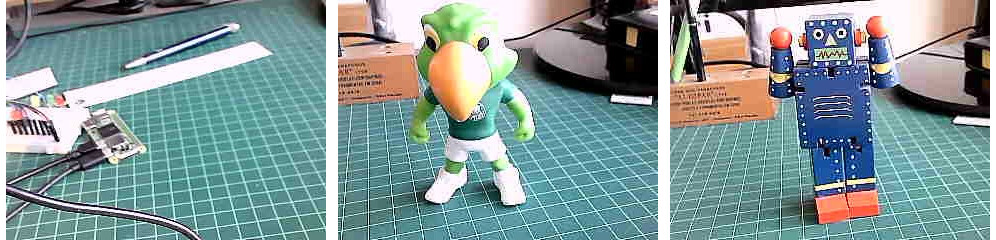
\includegraphics[width=0.72\textwidth]{images/day05/image_dataset_examples.jpg}
  \par\endgroup
  \vskip 0.2em
  \small
  \renewcommand{\arraystretch}{1.15}
  \begingroup\centering
  \begin{tabular}{@{}L{0.07\textwidth}L{0.70\textwidth}L{0.12\textwidth}@{}}
    \toprule
    \textbf{Step} & \textbf{Work} & \textbf{Time} \\
    \midrule
    1 & Data: a second project, upload the three folders of
        \code{image\_dataset/} & 10 min \\
    2 & Impulse: images of $96 \times 96$, the transfer learning block
      & 5 min \\
    3 & Train the model, and test it in the Studio & 15 min \\
    4 & Deploy: build the library, upload the sketch & 15 min \\
    5 & Test with the nine photos of \code{test\_images/} & 10 min \\
    \bottomrule
  \end{tabular}\par\endgroup
  \source{Three of the 81 photos of the dataset, with the classes
    \texttt{background}, \texttt{periquito}, and \texttt{robot}. Photos:
    repository EdgeML-with-Raspberry-Pi by Marcelo Rovai.}
\end{frame}

\begin{frame}{Part B: the settings in the Studio}
  \small
  \renewcommand{\arraystretch}{1.25}
  \begingroup\centering
  \begin{tabular}{@{}L{0.24\textwidth}L{0.66\textwidth}@{}}
    \toprule
    \textbf{Page} & \textbf{Setting} \\
    \midrule
    \code{Data acquisition} & Upload each folder with its label, with the
        automatic split. It is not an object detection project. \\
    \code{Create impulse} & Image size $96 \times 96$. Blocks: \code{Image}
        and \code{Transfer Learning (Images)}. \\
    \code{Image} & Colour depth \code{RGB}. Generate the features. \\
    \code{Transfer learning} & Model \code{MobileNetV2 96x96 0.35}, 16
        neurons in the last layer, dropout 0.1. 20 training cycles,
        learning rate 0.0005, data augmentation. \\
    \code{Model testing} & Classify all test images. \\
    \bottomrule
  \end{tabular}\par\endgroup
  \vskip 0.5em
  \begin{itemize}
    \item \textbf{You record:} the accuracy, and the estimates of the
          Studio for the inferencing time, the peak RAM, and the flash.
    \item Compare the peak RAM of the Studio with the peak of the lecture
          for this model: 135 KB.
  \end{itemize}
\end{frame}

\begin{frame}[fragile]{Part B: the test on the kit}
  \small
  Upload \code{sketches/image\_classifier/image\_classifier.ino}, with the
  header of your image library. The Serial Monitor shows for each frame:
\begin{lstlisting}
Predictions (DSP: ... ms., Classification: ... ms., Anomaly: ... ms.):
Timing (Capture: ... ms., Loop: ... ms.), free internal heap: ... bytes
Predictions:
  background: ...
  periquito: ...
  robot: ...
Best: ... (... %), display: ...
\end{lstlisting}
  \begin{itemize}
    \item Open the nine photos of \code{test\_images/} on the laptop
          screen, one after the other. Point the camera at the screen, so
          that the photo fills the image.
    \item The display shows a class only when three frames in sequence
          agree. Until then it shows \code{...}.
    \item Set \code{VOTE\_FRAMES} to 1, upload, and compare.
    \item \textbf{You record:} the class of the display for each photo,
          with the two settings.
  \end{itemize}
  \source{The output shows the form of the lines.}
\end{frame}

% ------------------------------------------------------------------- Part C
\begin{frame}{Part C: measure (15 min)}
  \small
  \renewcommand{\arraystretch}{1.25}
  \begingroup\centering
  \begin{tabular}{@{}L{0.26\textwidth}L{0.32\textwidth}L{0.32\textwidth}@{}}
    \toprule
    \textbf{Number} & \textbf{Keyword sketch} & \textbf{Image sketch} \\
    \midrule
    Capture time    & Not necessary & \code{Capture} \\
    Feature time    & \code{dsp\_ms} & \code{DSP} \\
    Inference time  & \code{classification\_ms} & \code{Classification} \\
    Complete loop   & \code{stride\_ms} & \code{Loop} \\
    Flash           & \code{Sketch uses ... bytes} of the build
                    & The same line \\
    RAM             & \code{Free heap}, and the peak RAM of the Studio
                    & \code{free internal heap}, and the peak RAM of the
                      Studio \\
    \bottomrule
  \end{tabular}\par\endgroup
  \vskip 0.5em
  \vskip 0.3em
  Write the median of 10 lines for each time. Compare each measured time
  with the estimate of the Studio.
  \begin{exerciseblock}
    \textbf{Prediction.} For which of the two models is the feature time
    larger than the inference time? Write your answer before you read the
    Serial Monitor.
  \end{exerciseblock}
\end{frame}
